\chapter{Greenhouse Software}
\label{chap:appendix}
%Reducing the spacing from the title


Here you write the context of the appendix, structuring such content in
sections, sub-sections and sub-sub-sections, if needed.

An example of appendix is the flat presentation of all the graphical user interface screens.
Each screen can be presented (identification symbol and description) and screens transition graph can be given.


\section{Login}
\label{sec:appendix_Login}
\begin{figure}
\includegraphics[width=1\textwidth]{images/mockup_login_eps.eps}
\end{figure}

The 'Login' page is the first page everyone sees before being able to use any
features of our software.

The User needs to identify himself with valid credentials.

\subsection{Username}
This input field is used for the \emph{Username} of the Gardener, Technician or
Manager.

\subsection{Password}
This input field is used for the \emph{Password} of the Gardener, Technician, or
Manager.

\subsection{Sign In Button}
This button send the request to be signed in, by clicking it.

\subsubsection{Success Scenario}
The \emph{User} is taken the \emph{Home} screen.

\subsubsection{Failure Scenario}
The \emph{User} gets a visible error message.





\section{Home}
\label{sec:appendix_Home}
\begin{figure}
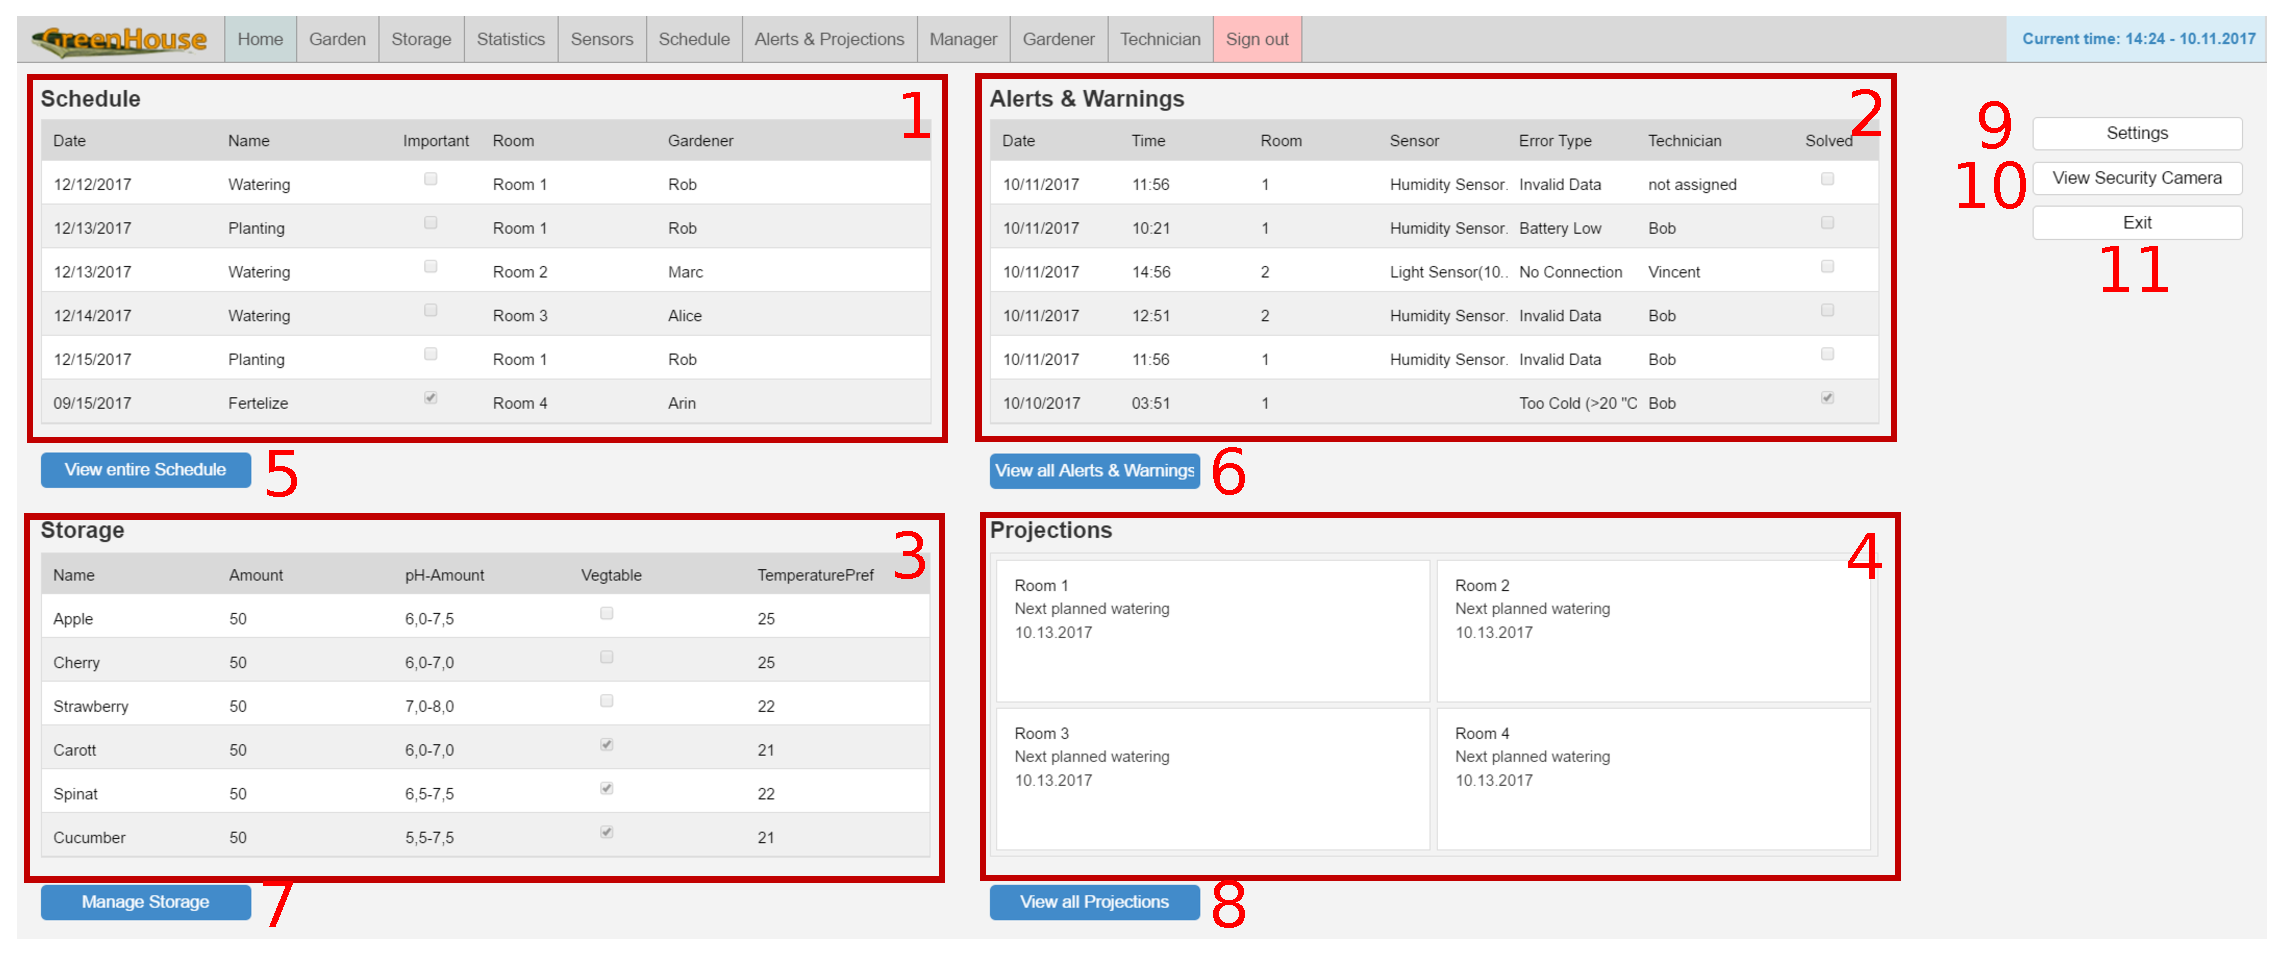
\includegraphics[width=1\textwidth]{images/mockup_home_eps.eps}
\end{figure}

The \emph{Home} page is the first page the \emph{User} sees after signing in.

This page gives a quick summary of the most important information about the most
recent alerts and warning, the next upcoming tasks and planned watering for each
room and low running stock. 

Further accesses through the blue and white buttons.

\subsection{Schedule}
The \emph{Schedule} shows a summary of the 6 next upcoming tasks of the
gardeners. The list contains information about the \emph{Date}, the \emph{Task
name}, the concerned \emph{Room} and \emph{Gardener} and a checkbox indicating
whether the task is \emph{Important}.

\subsection{Alerts and Warnings}
The \emph{Alerts and Warnings} list shows a summary of the 6 latest Alerts and
Warnings for the \emph{Technician}. The list contains information about the
\emph{Date} and \emph{Time} the alert or warning was added to the system, the
concerned \emph{Room} and \emph{Sensor} if there is a sensor assigned to the
alert or warning. The \emph{Error Type} gives more precise information about the
malfunctioning if it an alert. For Warnings is describes the Problem.
Additionally we get Information about the assigned \emph{Technician} if assigned
and if the problem is already \emph{Solved}.

\subsection{Storage}
The \emph{Storage} list shows a summary of the 6 items with the lowest quantity.
The list contains information about the \emph{Name} of the items, the current
\emph{Amount}. The other information about the \emph{pH-Amount, Vegetable and
TemperaturePref} are used to distinguish between more types of the same plant.

\subsection{Projections}
The \emph{Projections} grid shows a summary of the 4 next rooms planned
to be watered. The single grid contains informations about the concerned
\emph{Room} and the \emph{Date} for the next planned watering.

\subsection{View entire Schedule Button}
The \emph{View entire Schedule} button is a shortcut from the menu
\emph{Schedule} button. The button is designed for a fast access and has a blue
color.

\subsection{View all Alerst and Warnings Button}
The \emph{View all Alerts and Warnings} button is a shortcut from the menu
\emph{Alerts and Projections} button. The button is designed for a fast access
and has a blue color.

\subsection{Manage Storage Button}
The \emph{Manage Storage} button is a shortcut from the menu
\emph{Manager} button. The button is designed for a fast access and has a blue
color.

\subsection{View all Projections Button}
The \emph{View all Projections} button is a shortcut from the menu
\emph{Alerts and Projections} button. The button is designed for a fast access
and has a blue color.

\subsection{Settings Button}
The \emph{Settings} button opens a pop-up window with the \emph{Settings}
screen.

\subsection{View Security Camera Button}
The \emph{View Security Camera} button opens a pop-up window with the
\emph{Security Camera} screen.

\subsection{Exit Button}
The \emph{Exit} button signs the current \emph{User} out and closes the
\emph{Greenhouse} Software application.











\section{Manager Home screen}
\label{sec:appendix_Manager_Home_Screen}

\begin{figure}[H]
\includegraphics[width=1\textwidth]{images/FinalManagerHomeScreen.eps}
\end{figure}

The Manager home screen is the screen which is dedicated for his tasks most of
his features are executed here.


\subsection{Inventory of Seeds 29}
The table with the title Inventory of Seeds,displays all the content of seeds
left in the global inventory.

\subsection{Gardener retrives from Inventory 30}
The table with the title Gardener retrives from inventory displays at which time
a given gardener has retrived a given amount of seeds.

\subsection{Delete from Inventory of seeds 32}
This red button executes a function/ future which allows to remove a selected
seed completly from the sees inventory table.

\subsection{Go to manager home screeen}
This grey button can have 2 colors grey and red. By pressing the button the
manager gets redirected to the Manager request screen. In case the Button is red
the is a request that needs to be threated. If the button is Grey there is no
request but the manager can still go to the manager request screen.

\subsection{Add seed to Inventory Of Seeds 31}
This orange button executes a function/feature which allows to add a seed to 
the Inventory of Seeds. The input formula has to be completed before executing
the feature.


\subsubsection{Errors 31}
Constrains are on the textfields. In case of a wrong input look up the Error
Section of the user manual.





\section{Manager Request Screen}
\label{sec:appendix_Manager_Request_Screen}

\begin{figure}[H]
\includegraphics[width=1\textwidth]{images/FinalManagerRequestScreen.eps}
\end{figure}

The Manager Request screen is the screen which is dedicated to the request of an
Item from  Actors like the Gardener and the Technician or from the System. 


\subsection{Go to manager 1 screen 36}
This button redirects the manager to the Manager home screen.

\subsection{Ordering Seeds request by amount 35}
The manager can press the button arrow up or down for ascending or descening
order of the list.

\subsection{Accept requested seeds 34}
This green button allows the manager to execute a feature/function which accepts
a requested crop. 
\subsubsection{2 cases 34}
\tab{Request from the system automatically refills the the requested seeds.} 

\tab{Request from the Gardener the manager needs to add the requested crop by
it's own by adding a seed on the home screen.}

\subsection{Decline a seed Request 33}
This red button allows the manager to execute a function/feature which allows
him to decline a request for a seed.

\subsubsection{Errors 33}
Error can be thrown in case the request is 0.


\subsection{Decline a Sensor Request 38}
This red button allows the manager to execute a function/feature which allows
him to decline a request for a sensor.
\subsection{Decline a Sensor Request 37}
This green button executes a function/feature that allows to accept a request
for a sensor from the technican.





\section{Gardener Home Screen}
\label{sec:appendix_Gardener_Home_Screen}

\begin{figure}[H]
\includegraphics[width=1\textwidth]{images/GardenerHomeScreen.eps}
\end{figure}

The Gardener home screen is the main screen from the gardener all his
functionalities/features are present on this page.



\subsection{Seed inventory table 19}
This is a view of the global inventory seed in addtion the gardener can here
look up the temperature preference and the ph value needed for the planting.

\subsection{Modify Global seed inventory 17}
This geen modify button allows the gardener to retrive seeds from the inventory.
\subsubsection{Errors 17}
Constraints on the input it might occur due to wrong filling the input
formual an error might appear.

\subsection{Ask for non existing seeds 18}
This light red button allows the gardener to ask for a non exisitng seed. 


\subsection{Sensor table 16}
The table displays the temperature values from a given room which can be used
to plant seeds in the correct environment.

\subsection{Show my schedule 15 }
This blue button redirects the gardener to his schedule home screen.



\section{Technician Home Screen}
\label{sec:appendix_Technician_Home_Screen}

\begin{figure}[H]
\includegraphics[width=1\textwidth]{images/TechnicianHomeScreen.eps}
\end{figure}

The Technician home screen is the screen where the technician has all his
primary functionalities.



\subsection{Sensor Overview 40}
This is a drop down menu which allows the technician to categorize the sensors
by type and the system updates the table values.

\subsection{Modify Global seed inventory 43}
This orange button executes a function/feature which allows the technician to
ask for a new Sensor to the Manager.
\subsubsection{Errors 43}
In case the input formula is wrong completed an error might occur due to the
wrong input values.


\subsection{Request sensor table 42}
This red button allows the technician to remove a given sensor from the request
sensors list for any reason.This could happen due to adding a sensor or a
declination of the request (Where replacble is set to false).


























